\section{Experimentaci\'on 2}

\subsection{Red de oficina}

\subsubsection{Descripci\'on del contexto}
El experimento fue realizado en una red de ámbito laboral. Se trata de una pequeña empresa de desarrollo web que cuenta con 13 empleados, los cuales utilizan una computadora de escritorio o notebook además de dispositivos móviles.

\subsubsection{Descripci\'on de la captura}
Los resultados presentados a continuación se coresponden con la captura de paquetes de la red durante un intervalo de 3 horas.
Se capturó un total de 392521 paquetes, de los cuales 1715 fueron del tipo ARP.
\begin{itemize}
\item IP version 6: 3.67\%
\item ARP: 0.564\%
\item DOD Internet Protocol (IP): 95.7627%
\end{itemize}
Se puede observar que sólo se capturó 3 tipos de paquetes, de los cuales en su gran mayoría son del tipo DOD Internet Protocol (IP).
A contuniación se exhibe una comparación entre paquetes IP versión 6 y ARP, pudiendose observar que la cantidad de paquetes del tipo IP versión 6 es ampliamente mayor que la del tipo ARP.
\begin{center}
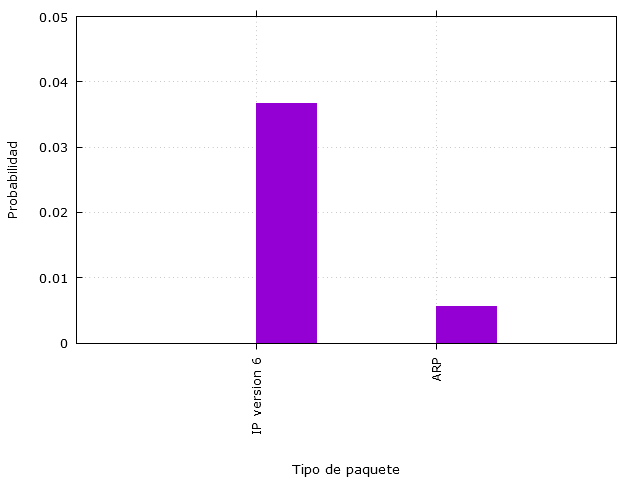
\includegraphics[width=0.5\textwidth]{exp2-graficos/grafico1exp2.png}
\end{center}

La entrop\'ia de la fuente S fue: 0.277044626815.\newline

Tomando los paquetes ARP se puede distinguir las direcciones IP en 34 diferentes, lo cual es un número razonable tiendo en cuenta la cantidad de terminales aproximada.

A continuación vemos un histograma con todas las direcciones IP observadas y la cantidad de paquetes hacia estas.

\begin{center}
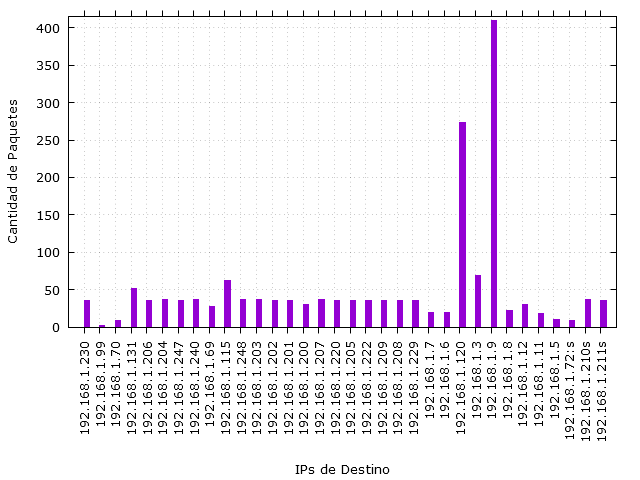
\includegraphics[width=0.75\textwidth]{exp2-graficos/grafico2exp2.png}
\end{center}

La entrop\'ia de la fuente S1 fue: 4.2739682572.


\subsubsection{An\'alisis de la captura}
